\documentclass[tikz,border=12pt]{standalone}
\usepackage[T1]{fontenc}
\usepackage{mathpazo}
\usepackage{amsmath,amssymb}
\usetikzlibrary{arrows.meta, positioning, calc, decorations.pathreplacing, patterns}

\definecolor{stblue}{HTML}{7B97AD}
\definecolor{rwgold}{HTML}{B8995E}
\definecolor{sage}{HTML}{7A9A7E}
\definecolor{dkbrown}{HTML}{3D3530}
\definecolor{wmgray}{HTML}{7B7067}
\definecolor{cream}{HTML}{F9F6F0}
\definecolor{border}{HTML}{D4C9B8}
\definecolor{terracotta}{HTML}{C47A6A}
\definecolor{lavender}{HTML}{907EA0}

\begin{document}
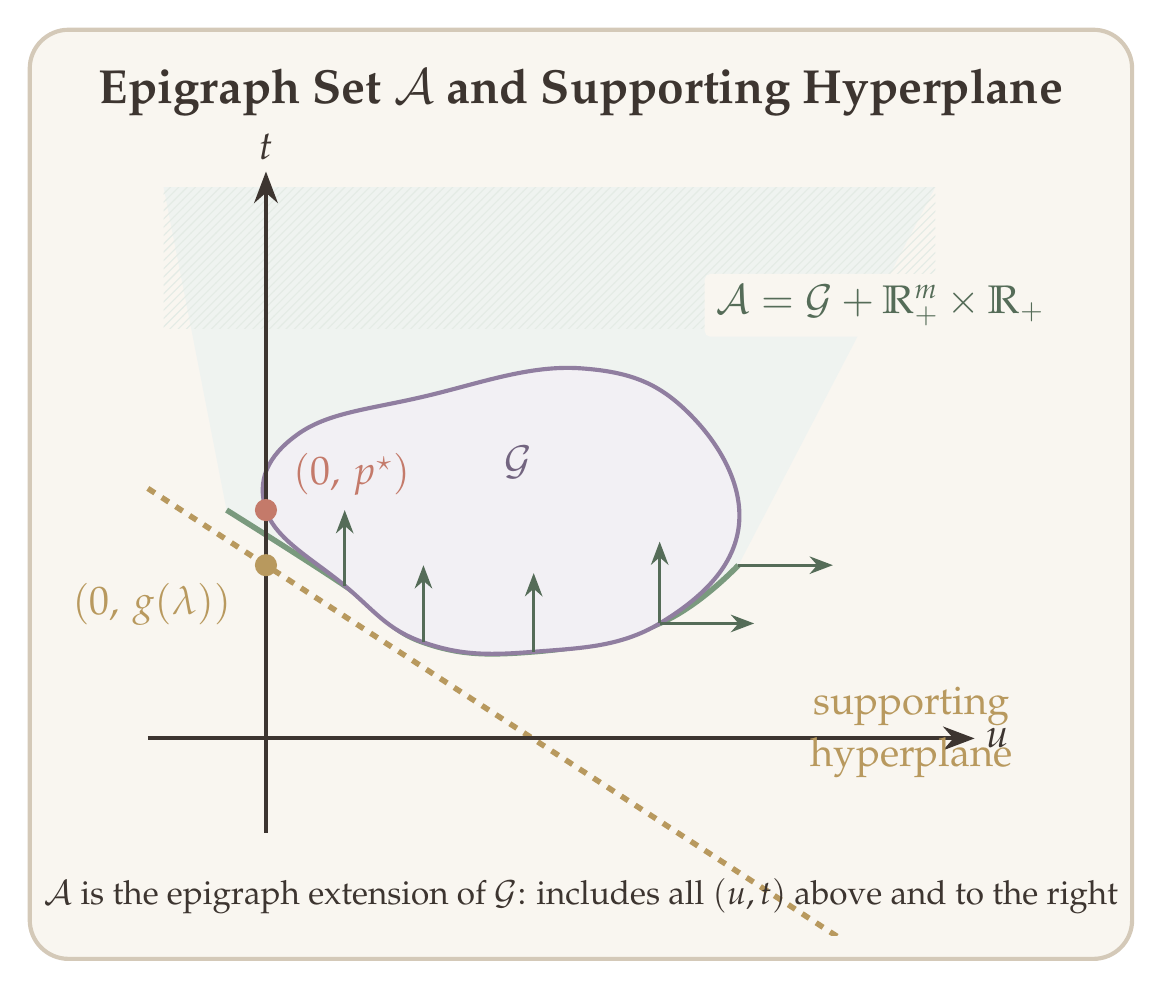
\begin{tikzpicture}[>={Stealth[length=4mm, width=3mm]}, line width=1.5pt]

% Background
\fill[cream, rounded corners=14pt] (-3.0,-2.8) rectangle (11,9);
\draw[border, line width=1.5pt, rounded corners=14pt] (-3.0,-2.8) rectangle (11,9);

% Title
\node[font=\LARGE\bfseries, text=dkbrown, align=center] at (4,8.2)
  {Epigraph Set $\mathcal{A}$ and Supporting Hyperplane};

% --- Fills and shapes (drawn BEFORE axes) ---

% Epigraph set A (upper-right extension of boundary of G)
\begin{scope}
\clip (-1.3,-0.8) rectangle (8.5,7);
\fill[sage!12]
  plot[smooth, tension=0.7] coordinates {
    (-0.5,2.9) (1,1.94) (2,1.22) (3.4,1.1) (5,1.46) (6,2.2)
  } -- (8.5,7) -- (-1.3,7) -- cycle;
\fill[pattern=north east lines, pattern color=sage!20]
  (-1.3,5.2) rectangle (8.5,7);
\draw[sage, line width=2pt]
  plot[smooth, tension=0.7] coordinates {
    (-0.5,2.9) (1,1.94) (2,1.22) (3.4,1.1) (5,1.46) (6,2.2)
  };
\end{scope}

% The set G -- overlaid as a smaller blob
\fill[lavender!12, draw=lavender, line width=1.5pt]
  plot[smooth cycle, tension=0.7] coordinates {
    (0,2.9) (1,1.94) (2,1.22) (3.4,1.1)
    (5,1.46) (6,2.66) (5.4,4.1)
    (4,4.7) (2,4.34) (0.4,3.86)
  };

% Supporting hyperplane of A (clipped to canvas)
\begin{scope}
\clip (-2,-2.5) rectangle (9,8);
\draw[rwgold, line width=2pt, dashed]
  (-1.5, {2.2+0.65*1.5}) -- (8.5, {2.2-0.65*8.5});
\end{scope}

% --- Axes (drawn AFTER fills so they remain visible) ---
\draw[->, dkbrown, line width=1.5pt] (-1.5,0) -- (9,0)
  node[right, font=\Large, text=dkbrown] {$u$};
\draw[->, dkbrown, line width=1.5pt] (0,-1.2) -- (0,7.2)
  node[above, font=\Large, text=dkbrown] {$t$};

% --- Labels and annotations ---

\node[font=\Large\bfseries, text=sage!80!black, fill=cream, inner sep=3pt, rounded corners=2pt] at (6,5.5) {$\mathcal{A}$};

% Small upward arrows at points on G's boundary to show extension direction
\draw[sage!70!black, line width=1.2pt, ->, >=Stealth] (1,1.94) -- (1,2.9);
\draw[sage!70!black, line width=1.2pt, ->, >=Stealth] (2,1.22) -- (2,2.2);
\draw[sage!70!black, line width=1.2pt, ->, >=Stealth] (3.4,1.1) -- (3.4,2.1);
\draw[sage!70!black, line width=1.2pt, ->, >=Stealth] (5,1.46) -- (5,2.5);
% Rightward arrows to show extension in u direction
\draw[sage!70!black, line width=1.2pt, ->, >=Stealth] (6,2.2) -- (7.2,2.2);
\draw[sage!70!black, line width=1.2pt, ->, >=Stealth] (5,1.46) -- (6.2,1.46);

\node[font=\Large\bfseries, text=lavender!80!black] at (3.2,3.5) {$\mathcal{G}$};

% Annotation for A = G + R^m_+ x R_+
\node[font=\Large, text=sage!70!black, align=center, fill=cream, inner sep=4pt, rounded corners=2pt] at (7.8,5.5)
  {$\mathcal{A} = \mathcal{G} + \mathbb{R}^m_+ \times \mathbb{R}_+$};

\node[font=\Large, text=rwgold] at (8.2,0.4) {supporting};
\node[font=\Large, text=rwgold] at (8.2,-0.25) {hyperplane};

% g(lambda) at u=0
\fill[rwgold] (0,2.2) circle (4pt);
\node[font=\Large\bfseries, text=rwgold, left] at (-0.3,1.7) {$(0,\, g(\lambda))$};

% p* at u=0
\fill[terracotta] (0,2.9) circle (4pt);
\node[font=\Large\bfseries, text=terracotta, right] at (0.2,3.35) {$(0,\, p^\star)$};

% Annotation
\node[font=\large, text=dkbrown, align=center] at (4,-2.0)
  {$\mathcal{A}$ is the epigraph extension of $\mathcal{G}$: includes all $(u,t)$ above and to the right};

\end{tikzpicture}
\end{document}
